\section{\ac{SAT}-solvers}

SMT vs. SAT is like high level \ac{PL} vs. assembly language.
The latter can be much more efficient, but it's hard to program in it.

SAT is abbreviation of ``Boolean satisfiability problem''.
The problem is to find such a set of variables, which, if plugged into boolean expression, will result in ``true''.

\subsection{CNF form}

\ac{CNF}\footnote{\url{https://en.wikipedia.org/wiki/Conjunctive_normal_form}} is a \textit{normal form}.

% TODO recheck
% TODO write abt it!
%\textit{normal form} is somewhat similar to polynomials in algebra. 
%What is polynomial?
%It is a standard way to express unsystematic equations like $2x \cdot x$ as $3x$ polynomial, 
%and so you will be able to apply some operations to polynomials like summing, etc.

Any boolean expression can be converted to \textit{normal form} and \ac{CNF} is one of them.
The \ac{CNF} expression is a bunch of clauses (sub-expressions) constisting of terms (variables), ORs and NOTs, 
all of which are then glueled together with AND into a full expression.
There is a way to memorize it: \ac{CNF} is ``AND of ORs'' (or ``product of sums'') and \ac{DNF} is ``OR of ANDs'' (or ``sum of products'').

Example is: $(\neg A \vee B) \wedge (C \vee \neg D)$.

$\vee$ stands for OR (logical disjunction\footnote{\url{https://en.wikipedia.org/wiki/Logical_disjunction}}), 
``+'' sign is also sometimes used for OR.

$\wedge$ stands for AND (logical conjunction\footnote{\url{https://en.wikipedia.org/wiki/Logical_conjunction}}).
It is easy to memorize: $\wedge$ looks like ``A'' letter.
``$\cdot$'' is also sometimes used for AND.

$\neg$ is negation (NOT).

% TODO A/B is the first clause, C/D is second

\subsection{Example: 2-bit adder}
\label{adder}

\ac{SAT}-solver is merely a solver of huge boolean equations in CNF form.
It just gives the answer, if there is a set of input values which can satisfy CNF expression, and what input values must be.

Here is a 2-bit adder for example:

\begin{figure}[ht!]
\centering
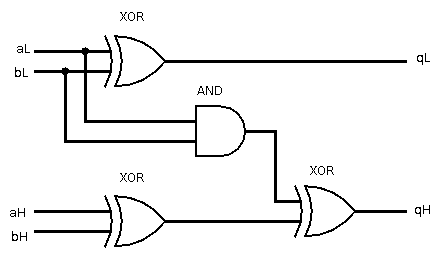
\includegraphics[scale=0.75]{SAT/adder_logisim.png}
\caption{2-bit adder circuit}
\end{figure}

The adder in its simplest form: it has no carry-in and carry-out, and it has 3 XOR gates and one AND gate.
Let's try to figure out, which sets of input values will force adder to set both two output bits?
By doing quick memory calculation, we can see that there are 4 ways to do so: $0+3=3$, $1+2=3$, $2+1=3$, $3+0=3$.
Here is also truth table, with these rows highlighted:

\newcommand{\HLcell}{\cellcolor{blue!25}}

\begin{center}
\begin{doublespace}
\noindent\(\begin{array}{l|llllll}
  & \text{aH} & \text{aL} & \text{bH} & \text{bL} & \text{qH} & \text{qL} \\
\hline
 \text{3+3 = 6 $\equiv $ 2 (mod 4)} & 1 & 1 & 1 & 1 & 1 & 0 \\
 \text{3+2 = 5 $\equiv $ 1 (mod 4)} & 1 & 1 & 1 & 0 & 0 & 1 \\
 \text{3+1 = 4 $\equiv $ 0 (mod 4)} & 1 & 1 & 0 & 1 & 0 & 0 \\
 \text{\HLcell{}3+0 = 3 $\equiv $ 3 (mod 4)} & \HLcell{}1 & \HLcell{}1 & \HLcell{}0 & \HLcell{}0 & \HLcell{}1 & \HLcell{}1 \\
 \text{2+3 = 5 $\equiv $ 1 (mod 4)} & 1 & 0 & 1 & 1 & 0 & 1 \\
 \text{2+2 = 4 $\equiv $ 0 (mod 4)} & 1 & 0 & 1 & 0 & 0 & 0 \\
 \text{\HLcell{}2+1 = 3 $\equiv $ 3 (mod 4)} & \HLcell{}1 & \HLcell{}0 & \HLcell{}0 & \HLcell{}1 & \HLcell{}1 & \HLcell{}1 \\
 \text{2+0 = 2 $\equiv $ 2 (mod 4)} & 1 & 0 & 0 & 0 & 1 & 0 \\
 \text{1+3 = 4 $\equiv $ 0 (mod 4)} & 0 & 1 & 1 & 1 & 0 & 0 \\
 \text{\HLcell{}1+2 = 3 $\equiv $ 3 (mod 4)} & \HLcell{}0 & \HLcell{}1 & \HLcell{}1 & \HLcell{}0 & \HLcell{}1 & \HLcell{}1 \\
 \text{1+1 = 2 $\equiv $ 2 (mod 4)} & 0 & 1 & 0 & 1 & 1 & 0 \\
 \text{1+0 = 1 $\equiv $ 1 (mod 4)} & 0 & 1 & 0 & 0 & 0 & 1 \\
 \text{\HLcell{}0+3 = 3 $\equiv $ 3 (mod 4)} & \HLcell{}0 & \HLcell{}0 & \HLcell{}1 & \HLcell{}1 & \HLcell{}1 & \HLcell{}1 \\
 \text{0+2 = 2 $\equiv $ 2 (mod 4)} & 0 & 0 & 1 & 0 & 1 & 0 \\
 \text{0+1 = 1 $\equiv $ 1 (mod 4)} & 0 & 0 & 0 & 1 & 0 & 1 \\
 \text{0+0 = 0 $\equiv $ 0 (mod 4)} & 0 & 0 & 0 & 0 & 0 & 0 \\
\end{array}\)
\end{doublespace}
\end{center}


Let's find, what \ac{SAT}-solver can say about it?

First, we should represent our 2-bit adder as \ac{CNF} expression.

Using Wolfram Mathematica, we can express 1-bit expression for both adder outputs:\\
\\
\textbf{\texttt{In[]:=AdderQ0[aL$\_$,bL$\_$]=Xor[aL,bL]}} \\
\textbf{\texttt{Out[]:=aL $\veebar$ bL}} \\
\\
\textbf{\texttt{In[]:=AdderQ1[aL$\_$,aH$\_$,bL$\_$,bH$\_$]=Xor[And[aL,bL],Xor[aH,bH]]}} \\
\textbf{\texttt{Out[]:=aH $\veebar$ bH $\veebar$ (aL \&\& bL)}} \\
\\
We need such expression, where both parts will generate 1's.
Let's use Wolfram Mathematica find all instances of such expression (I glueled both parts with And): \\
\\
\textbf{\texttt{In[]:=Boole[SatisfiabilityInstances[And[AdderQ0[aL,bL],AdderQ1[aL,aH,bL,bH]],\{aL,aH,bL,bH\},4]]}} \\
\textbf{\texttt{Out[]:=\{1,1,0,0\},\{1,0,0,1\},\{0,1,1,0\},\{0,0,1,1\}}} \\
\\
Yes, indeed, Mathematica says, there are 4 inputs which will lead to the result we need.
So, Mathematica can also be used as \ac{SAT} solver.

Nevertheless, let's proceed to \ac{CNF} form. Using Mathematica again, let's convert our expression to \ac{CNF} form:\\
\\
\textbf{\texttt{In[]:=cnf=BooleanConvert[And[AdderQ0[aL,bL],AdderQ1[aL,aH,bL,bH]],``CNF'']}} \\
\textbf{\texttt{Out[]:=(!aH $\|$ !bH) \&\& (aH $\|$ bH) \&\& (!aL $\|$ !bL) \&\& (aL $\|$ bL)}} \\
\\
Looks more complex. The reason of such verbosity is that \ac{CNF} form doesn't allow XOR operations.
% FIXME: TeX form of the expression!

\subsubsection{MiniSat}

For starters, we can try MiniSat\footnote{\url{http://minisat.se/MiniSat.html}}.
The standard way to encode \ac{CNF} expression for MiniSat is to enumerate all OR parts at each line.
Also, MiniSat doesn't support variable names, just numbers.
Let's enumerate our variables: 1 will be aH, 2 -- aL, 3 -- bH, 4 -- bL.

Here is what I've got when I converted Mathematica expression to the MiniSat input file:

\lstinputlisting{SAT/adder.cnf}

Two 4's at the first lines are number of variables and number of clauses respectively.
There are 4 lines then, each for each OR clause.
Minus before variable number meaning that the variable is negated.
Absence of minus -- not negated.
Zero at the end is just terminating zero, meaning end of the clause.

In other words, each line is OR-clause with optional negations,
and the task of MiniSat is to find such set of input, which can satisfy all lines in the input file.

That file I named as \textit{adder.cnf} and now let's try MiniSat:

\begin{lstlisting}
% minisat -verb=0 adder.cnf results.txt
SATISFIABLE
\end{lstlisting}

The results are in \textit{results.txt} file:

\begin{lstlisting}
SAT
-1 -2 3 4 0
\end{lstlisting}

This means, if the first two variables (aH and aL) will be \textit{false}, and the last two variables (bH and bL) will be set to \textit{true},
the whole \ac{CNF} expression is satisfiable.
Seems to be true: if bH and bL are the only inputs set to \textit{true}, both resulting bits are also has \textit{true} states.

Now how to get other instances? \ac{SAT}-solvers, like \ac{SMT} solvers, produce only one solution (or \textit{instance}).

MiniSat uses \ac{PRNG} and its initial seed can be set explicitely. I tried different values, but result is still the same.
Nevertheless, CryptoMiniSat in this case was able to show all possible 4 instances, in chaotic order, though.
So this is not very robust way.

Perhaps, the only known way is to negate solution clause and add it to the input expression.
We've got \TT{-1 -2 3 4}, 
now we can negate all values in it (just toggle minuses: \TT{1 2 -3 -4}) and add it to the end of the input file:

\begin{lstlisting}
p cnf 4 5
-1 -3 0
1 3 0
-2 -4 0
2 4 0
1 2 -3 -4
\end{lstlisting}

Now we've got another result:

\begin{lstlisting}
SAT
1 2 -3 -4 0
\end{lstlisting}

This means, aH and aL must be both \textit{true} and bH and bL must be \textit{false}, to satisfy the input expression.
Let's negate this clause and add it again:

\begin{lstlisting}
p cnf 4 6
-1 -3 0
1 3 0
-2 -4 0
2 4 0
1 2 -3 -4
-1 -2 3 4 0
\end{lstlisting}

The result is:

\begin{lstlisting}
SAT
-1 2 3 -4 0
\end{lstlisting}

aH=false, aL=true, bH=true, bL=false. This is also correct, according to our truth table.

Let's add it again:

\begin{lstlisting}
p cnf 4 7
-1 -3 0
1 3 0
-2 -4 0
2 4 0
1 2 -3 -4
-1 -2 3 4 0
1 -2 -3 4 0
\end{lstlisting}

\begin{lstlisting}
SAT
1 -2 -3 4 0
\end{lstlisting}

\textit{aH=true, aL=false, bH=false, bL=true.} This is also correct.

This is fourth result. There are shouldn't be more. What if to add it?

\begin{lstlisting}
p cnf 4 8
-1 -3 0
1 3 0
-2 -4 0
2 4 0
1 2 -3 -4
-1 -2 3 4 0
1 -2 -3 4 0
-1 2 3 -4 0
\end{lstlisting}

Now MiniSat just says ``UNSATISFIABLE'' without any additional information in the resulting file.

Our example is tiny, but MiniSat can work with huge \ac{CNF} expressions.

\subsubsection{CryptoMiniSat}

XOR operation is absent in \ac{CNF} form, but crucial in cryptographical algorithms.
Simplest possible way to represent single XOR operation in \ac{CNF} form is:
$(\neg x \vee \neg y) \wedge (x \vee y)$ -- not that small expression, 
though, many XOR operations in single expression can be optimized better.

One significant difference between MiniSat and CryptoMiniSat is that
the latter supports clauses with XOR operations instead of ORs,
because CryptoMiniSat has aim to analyze crypto algorithms\footnote{\url{http://www.msoos.org/xor-clauses/}}.
XOR clauses are handled by CryptoMiniSat in a special way without translating to OR clauses.

You need just to prepend a clause with ``x'' in \ac{CNF} file and OR clause is then treated as XOR clause by CryptoMiniSat.
As of 2-bit adder, this smallest possible XOR-CNF expression can be used to find all inputs where both output adder bits are set:

$(aH \oplus bH) \wedge (aL \oplus bL)$

This is \TT{.cnf} file for CryptoMiniSat:

\begin{lstlisting}
p cnf 4 2
x1 3 0
x2 4 0
\end{lstlisting}

Now I run CryptoMiniSat with various random values to initialize its \ac{PRNG} \dots

\begin{lstlisting}
% cryptominisat4 --verb 0 --random 0 XOR_adder.cnf
s SATISFIABLE
v 1 2 -3 -4 0
% cryptominisat4 --verb 0 --random 1 XOR_adder.cnf
s SATISFIABLE
v -1 -2 3 4 0
% cryptominisat4 --verb 0 --random 2 XOR_adder.cnf
s SATISFIABLE
v 1 -2 -3 4 0
% cryptominisat4 --verb 0 --random 3 XOR_adder.cnf
s SATISFIABLE
v 1 2 -3 -4 0
% cryptominisat4 --verb 0 --random 4 XOR_adder.cnf
s SATISFIABLE
v -1 2 3 -4 0
% cryptominisat4 --verb 0 --random 5 XOR_adder.cnf
s SATISFIABLE
v -1 2 3 -4 0
% cryptominisat4 --verb 0 --random 6 XOR_adder.cnf
s SATISFIABLE
v -1 -2 3 4 0
% cryptominisat4 --verb 0 --random 7 XOR_adder.cnf
s SATISFIABLE
v 1 -2 -3 4 0
% cryptominisat4 --verb 0 --random 8 XOR_adder.cnf
s SATISFIABLE
v 1 2 -3 -4 0
% cryptominisat4 --verb 0 --random 9 XOR_adder.cnf
s SATISFIABLE
v 1 2 -3 -4 0
\end{lstlisting}

Nevertheless, all 4 possible solutions are:

\begin{lstlisting}
v -1 -2 3 4 0
v -1 2 3 -4 0
v 1 -2 -3 4 0
v 1 2 -3 -4 0
\end{lstlisting}

\dots the same as reported by MiniSat.

\subsection{Picosat}

At least Picosat can enumerate all possible solutions without crutches I just shown:

\begin{lstlisting}
% picosat --all adder.cnf
s SATISFIABLE
v -1 -2 3 4 0
s SATISFIABLE
v -1 2 3 -4 0
s SATISFIABLE
v 1 2 -3 -4 0
s SATISFIABLE
v 1 -2 -3 4 0
s SOLUTIONS 4
\end{lstlisting}

% subsections:
\subsection{Eight queens puzzle}
\label{EightQueens}

Eight queens is a very popular puzzle and often used for measuring performance of SAT solvers.
The problem is to place 8 queens on chess board so they will not attack each other.
For example:

\begin{lstlisting}
| | | |*| | | | |
| | | | | | |*| |
| | | | |*| | | |
| |*| | | | | | |
| | | | | |*| | |
|*| | | | | | | |
| | |*| | | | | |
| | | | | | | |*|
\end{lstlisting}

Let's try to figure out how to solve it.

\subsubsection{POPCNT1}
\label{POPCNTOne}

One important function we will (often) use is \TT{POPCNT1}.
This is a function which returns \textit{True} if one single of inputs is \textit{True} and others are \textit{False}.
It will return \textit{False} otherwise.

In my other examples, I've used Wolfram Mathematica to generate CNF clauses for it, for example: \ref{minesweeper_SAT}.
What expression Mathematica offers as \TT{POPCNT1} function with 8 inputs?

\begin{lstlisting}
(!a||!b)&&(!a||!c)&&(!a||!d)&&(!a||!e)&&(!a||!f)&&(!a||!g)&&(!a||!h)&&(a||b||c||d||e||f||g||h)&&
(!b||!c)&&(!b||!d)&&(!b||!e)&&(!b||!f)&&(!b||!g)&&(!b||!h)&&(!c||!d)&&(!c||!e)&&(!c||!f)&&(!c||!g)&&
(!c||!h)&&(!d||!e)&&(!d||!f)&&(!d||!g)&&(!d||!h)&&(!e||!f)&&(!e||!g)&&(!e||!h)&&(!f||!g)&&(!f||!h)&&(!g||!h)
\end{lstlisting}

We can clearly see that the expression constisting of all possible variable pairs (negated) plus
enumeration of all variables (non-negated).
In plain English terms, this means: ``no pair can be equal to two \textit{True}'s \textit{AND} at least one \textit{True}
must be present among all variables''.

This is how it works: if two variables will be \textit{True}, negated they will be both \textit{False},
and this clause will not be evaluated
to \textit{True}, which is our ultimate goal.
If one of variables is \textit{True}, both negated will produce one \textit{True} and one \textit{False} (fine).
If both variables are False, both negated will produce two \textit{True's} (again, fine).

Here is how I can generate clauses for the function using \textit{itertools} module from Python,
which provides many important functions from combinatorics:

\begin{lstlisting}
    # naive/pairwise encoding   
    def AtMost1(self, lst):
        for pair in itertools.combinations(lst, r=2):
            self.add_clause([self.neg(pair[0]), self.neg(pair[1])])
        
    def POPCNT1(self, lst):
        self.AtMost1(lst)
        self.OR_always(lst)
\end{lstlisting}

\TT{AtMost1()} function enumerates all possible pairs using \textit{itertools} function
\textit{combinations()}.

\TT{POPCNT1()} function does the same, but also adds a final clause, which forces at least one
\textit{True} variable to be present.

What clauses will be generated for 5 variables (1..5)?

\lstinputlisting{SAT/8queens/popcnt1.cnf}

Yes, these are all possible pairs of 1..5 numbers + all 5 numbers.

We can get all solutions using Picosat:

\begin{lstlisting}
% picosat --all popcnt1.cnf
s SATISFIABLE
v -1 -2 -3 -4 5 0
s SATISFIABLE
v -1 -2 -3 4 -5 0
s SATISFIABLE
v -1 -2 3 -4 -5 0
s SATISFIABLE
v -1 2 -3 -4 -5 0
s SATISFIABLE
v 1 -2 -3 -4 -5 0
s SOLUTIONS 5
\end{lstlisting}

5 possible solutions indeed.

\subsubsection{Eight queens}

Now let's get back to eight queens.

We can assign 64 variables to $8 \cdot 8=64$ cells.
Cell occuppied with queen will be \textit{True}, vacant cell will be \textit{False}.

The problem of placing non-attacking (each other) queens on chess board (of any size) can be stated in plain English like this:
\begin{itemize}
\item one single queen must be present at each row;

\item one single queen must be present at each column;

\item zero or one queen must be present at each diagonal (empty diagonals can be present in valid solution).
\end{itemize}

These rules can be translated like that:

\begin{itemize}
\item POPCNT1(each row)==\textit{True}

\item POPCNT1(each column)==\textit{True}

\item AtMost1(each diagonal)==\textit{True}
\end{itemize}

Now all we need is to enumerate rows, columns and diagonals and gather all clauses:

\lstinputlisting{SAT/8queens/8queens.py}
( \url{https://github.com/DennisYurichev/SAT_SMT_article/blob/master/SAT/8queens/8queens.py} )

Perhaps, \TT{gen\_diagonal()} function is not very aesthetically appealing: it enumerates also subdiagonals
of already enumerated longer diagonals.
To prevent presence of duplicate clauses, \textit{clauses} global variable is not a list, rather set, which allows
only unique data to be present there.

Also, I've used \TT{AtMost1} for each column, this will help to produce slightly lower number of clauses.
Each column will have a queen anyway, this is implied from the first rule (\TT{POPCNT1} for each row).

After running, we got CNF file with 64 variables and 736 clauses (\url{https://github.com/DennisYurichev/SAT_SMT_article/blob/master/SAT/8queens/8queens.cnf}).
Here is one solution:

\begin{lstlisting}
% python 8queens.py
len(clauses)= 736
| | | |*| | | | |
| | | | | | |*| |
| | | | |*| | | |
| |*| | | | | | |
| | | | | |*| | |
|*| | | | | | | |
| | |*| | | | | |
| | | | | | | |*|
\end{lstlisting}

How many possible solutions are there?
Picosat tells 92, which is indeed correct number of solutions (\url{https://oeis.org/A000170}).

Performance of Picosat is not impressive, probably because it has to output all the solutions.
It took 34 seconds on my ancient Intel Atom 1.66GHz netbook to enumerate all solutions for $11 \cdot 11$ chess board
(2680 solutions),
which is way slower than my straigt brute-force program: \url{https://yurichev.com/blog/8queens/}.
Nevertheless, it's lighting fast (as other SAT solvers) in finding first solution.

The SAT instance is also small enough to be easily solved by my simplest possible backtracking SAT solver:
\ref{SAT_backtrack}.

\subsubsection{Counting all solutions}

We get a solution, negate it and add as a new constraint.
In plain English language this sounds ``find a solution, which is also can't be equal to the recently found/added''.
We add them consequently and the process is slowing---just because a problem (\textit{instance}) is growing and SAT solver
experience hard times in find yet another solution.

\subsubsection{Skipping symmetrical solutions}

We can also add rotated and reflected (horizontally) solution, so to skip symmetrical solutions.
By doing so, we're getting 12 solutions for 8*8 board, 46 for 9*9 board, etc.
This is \url{https://oeis.org/A002562}.


\subsection{Simplest SAT solver in \textasciitilde{}120 lines}
\label{SAT_backtrack}

This is simplest possible backtracking SAT solver written in Python (not a \ac{DPLL} one).
It uses the same backtracking algorithm you can find in many simple Sudoku and 8 queens solvers.
It works significantly slower, but due to its extreme simplicity, it can also count solutions.
For example, it can count all solutions of 8 queens problem (\ref{EightQueens}).

Also, there are 70 solutions for POPCNT4 function
\footnote{\url{https://github.com/DennisYurichev/SAT_SMT_article/blob/master/SAT/backtrack/POPCNT4.cnf}}
(the function is true if any 4 of its input 8 variables are true):

\begin{lstlisting}
SAT
-1 -2 -3 -4 5 6 7 8 0
SAT
-1 -2 -3 4 -5 6 7 8 0
SAT
-1 -2 -3 4 5 -6 7 8 0
SAT
-1 -2 -3 4 5 6 -7 8 0
...

SAT
1 2 3 -4 -5 6 -7 -8 0
SAT
1 2 3 -4 5 -6 -7 -8 0
SAT
1 2 3 4 -5 -6 -7 -8 0
UNSAT
solutions= 70
\end{lstlisting}

It was also tested on my SAT-based Minesweeper cracker (\ref{minesweeper_SAT}),
and finishes in reasonable time (though, slower than MiniSat by a factor of \textasciitilde{}10).

On bigger \ac{CNF} instances, it gets stuck, though.

The source code:

\lstinputlisting{SAT/backtrack/SAT_backtrack.py}

As you can see, all it does is enumerate all possible solutions, but prunes search tree as early as possible.
This is backtracking.

The files: \url{https://github.com/DennisYurichev/SAT_SMT_article/tree/master/SAT/backtrack}.

Some comments: \url{https://www.reddit.com/r/compsci/comments/6jn3th/simplest_sat_solver_in_120_lines/}.


\subsection{Pocket Rubik's Cube (2*2*2) and SAT solver}
\label{PocketCubeSAT}.

I had success with my SAT-based solver, which can find an 11-turn path for a matter of 10-20 minutes on my old
Intel Xeon E3-1220 3.10GHz.

First, we will encode each color as 3-bit bit vector.
Then we can build electronic circuit, which will take initial state of cube and output final state.
It can have switches for each turn on each state.

% TODO TikZ
\begin{lstlisting}
                 +-----+    +-----+     +-----+
initial state -> | blk | -> | blk | ... | blk | -> final state
                 +-----+    +-----+     +-----+
                    ^          ^           ^
                    |          |           |
                  turn 1     turn 2    last turn
\end{lstlisting}

You set all turns and the device "calculates" final state.

Each "blk" can be constisted of 24 multiplexers (MUX), each for each facelet.
Each MUX is controlled by 5-bit command (turn number).
Depending on command, MUX takes 3-bit color from a facelet from a previous state.

Here is a table: the first column is a "destination" facelet, then a list of "source" facelets for each turn:

\begin{lstlisting}
    #      dst,  FCW  FH   FCCW UCW  UH   UCCW DCW  DH   DCCW RCW  RH   RCCW LCW  LH   LCCW BCW  BH   BCCW
    add_r("F1",["F3","F4","F2","R1","B1","L1","F1","F1","F1","F1","F1","F1","U1","B4","D1","F1","F1","F1"])
    add_r("F2",["F1","F3","F4","R2","B2","L2","F2","F2","F2","D2","B3","U2","F2","F2","F2","F2","F2","F2"])
    add_r("F3",["F4","F2","F1","F3","F3","F3","L3","B3","R3","F3","F3","F3","U3","B2","D3","F3","F3","F3"])
    add_r("F4",["F2","F1","F3","F4","F4","F4","L4","B4","R4","D4","B1","U4","F4","F4","F4","F4","F4","F4"])
    add_r("U1",["U1","U1","U1","U3","U4","U2","U1","U1","U1","U1","U1","U1","B4","D1","F1","R2","D4","L3"])
    add_r("U2",["U2","U2","U2","U1","U3","U4","U2","U2","U2","F2","D2","B3","U2","U2","U2","R4","D3","L1"])
    add_r("U3",["L4","D2","R1","U4","U2","U1","U3","U3","U3","U3","U3","U3","B2","D3","F3","U3","U3","U3"])
    add_r("U4",["L2","D1","R3","U2","U1","U3","U4","U4","U4","F4","D4","B1","U4","U4","U4","U4","U4","U4"])
    add_r("D1",["R3","U4","L2","D1","D1","D1","D3","D4","D2","D1","D1","D1","F1","U1","B4","D1","D1","D1"])
    add_r("D2",["R1","U3","L4","D2","D2","D2","D1","D3","D4","B3","U2","F2","D2","D2","D2","D2","D2","D2"])
    add_r("D3",["D3","D3","D3","D3","D3","D3","D4","D2","D1","D3","D3","D3","F3","U3","B2","L1","U2","R4"])
    add_r("D4",["D4","D4","D4","D4","D4","D4","D2","D1","D3","B1","U4","F4","D4","D4","D4","L3","U1","R2"])
    add_r("R1",["U3","L4","D2","B1","L1","F1","R1","R1","R1","R3","R4","R2","R1","R1","R1","R1","R1","R1"])
    add_r("R2",["R2","R2","R2","B2","L2","F2","R2","R2","R2","R1","R3","R4","R2","R2","R2","D4","L3","U1"])
    add_r("R3",["U4","L2","D1","R3","R3","R3","F3","L3","B3","R4","R2","R1","R3","R3","R3","R3","R3","R3"])
    add_r("R4",["R4","R4","R4","R4","R4","R4","F4","L4","B4","R2","R1","R3","R4","R4","R4","D3","L1","U2"])
    add_r("L1",["L1","L1","L1","F1","R1","B1","L1","L1","L1","L1","L1","L1","L3","L4","L2","U2","R4","D3"])
    add_r("L2",["D1","R3","U4","F2","R2","B2","L2","L2","L2","L2","L2","L2","L1","L3","L4","L2","L2","L2"])
    add_r("L3",["L3","L3","L3","L3","L3","L3","B3","R3","F3","L3","L3","L3","L4","L2","L1","U1","R2","D4"])
    add_r("L4",["D2","R1","U3","L4","L4","L4","B4","R4","F4","L4","L4","L4","L2","L1","L3","L4","L4","L4"])
    add_r("B1",["B1","B1","B1","L1","F1","R1","B1","B1","B1","U4","F4","D4","B1","B1","B1","B3","B4","B2"])
    add_r("B2",["B2","B2","B2","L2","F2","R2","B2","B2","B2","B2","B2","B2","D3","F3","U3","B1","B3","B4"])
    add_r("B3",["B3","B3","B3","B3","B3","B3","R3","F3","L3","U2","F2","D2","B3","B3","B3","B4","B2","B1"])
    add_r("B4",["B4","B4","B4","B4","B4","B4","R4","F4","L4","B4","B4","B4","D1","F1","U1","B2","B1","B3"])
\end{lstlisting}

Each MUX has 32 inputs, each has width of 3 bits: colors from "source" facelets.
It has 3-bit output (color for "destination" facelet).
It has 5-bit selector, for 18 turns. Other selector values (32-18=14 values) are not used at all.

The whole problem is to build a circuit and then ask SAT solver to set "switches" to such a state,
when input and output are determined (by us).

Now the problem is to represent MUX in CNF terms.

From \ac{EE} courses we can remember about a simple if-then-else (ITE) gate, it takes 3 inputs
("selector", "true" and "false") and it has 1 output.
Depending on "selector" input it "connects" output with "true" or "false" input.
Using tree of ITE gates we first can build 32-to-1 MUX, then wide 32*3-to-3 MUX.

% FIXME URL
I once have written small utility to search for shortest possible CNF formula for a specific function,
in a bruteforce manner (\url{https://github.com/DennisYurichev/yurichev.com/blob/master/blog/rubik/XOR_CNF_bf.c}).
It was inspired by "aha! hacker assistant" by Henry Warren.
So here is a function:

\begin{lstlisting}
bool func(bool v[VARIABLES])
{

	// ITE:

	bool tmp;
	if (v[0]==0)
		tmp=v[1];
	else
		tmp=v[2];

	return tmp==v[3];
}
\end{lstlisting}

A shortest CNF for it:

\begin{lstlisting}
try_all_CNFs_of_len(1)
try_all_CNFs_of_len(2)
try_all_CNFs_of_len(3)
try_all_CNFs_of_len(4)
found a CNF:
p cnf 4 4
-1 3 -4 0
1 2 -4 0
-1 -3 4 0
1 -2 4 0
\end{lstlisting}

1st variable is "select", 2nd is "false", 3rd is "true", 4th is "output".
"output" is an additional variable, added just like in Tseitin transformations.

Hence, CNF formula is:

\begin{lstlisting}
(!select OR true OR !output) AND (select OR false OR !output) AND (!select OR !true OR output) AND (select OR !false OR output)
\end{lstlisting}

It assures that the "output" will always be equal to one of inputs depending on "select".

Now we can build a tree of ITE gates:

\begin{lstlisting}
def create_ITE(s,f,t):
    x=create_var()

    clauses.append([neg(s),t,neg(x)])
    clauses.append([s,f,neg(x)])
    clauses.append([neg(s),neg(t),x])
    clauses.append([s,neg(f),x])

    return x

# ins=16 bits
# sel=4 bits
def create_MUX(ins, sel):
    t0=create_ITE(sel[0],ins[0],ins[1])
    t1=create_ITE(sel[0],ins[2],ins[3])
    t2=create_ITE(sel[0],ins[4],ins[5])
    t3=create_ITE(sel[0],ins[6],ins[7])
    t4=create_ITE(sel[0],ins[8],ins[9])
    t5=create_ITE(sel[0],ins[10],ins[11])
    t6=create_ITE(sel[0],ins[12],ins[13])
    t7=create_ITE(sel[0],ins[14],ins[15])

    y0=create_ITE(sel[1],t0,t1)
    y1=create_ITE(sel[1],t2,t3)
    y2=create_ITE(sel[1],t4,t5)
    y3=create_ITE(sel[1],t6,t7)

    z0=create_ITE(sel[2],y0,y1)
    z1=create_ITE(sel[2],y2,y3)

    return create_ITE(sel[3], z0, z1)
\end{lstlisting}

This is my old MUX I wrote for 16 inputs and 4-bit selector, but you've got the idea: this is 4-tier tree.
It has 15 ITE gates or 15*4=60 clauses.

Now the question, is it possible to make it smaller?
I've tried to use Mathematica.
First I've built truth table for 4-bit selector:

\begin{lstlisting}
...
1 1 1 1     1 1 1 1 1 1 0 1 0 1 0 1 1 0 1 1    0    0
1 1 1 1     1 1 1 1 1 1 0 1 0 1 0 1 1 0 1 1    1    1
1 1 1 1     1 1 1 1 1 1 0 1 0 1 0 1 1 1 0 0    0    0
1 1 1 1     1 1 1 1 1 1 0 1 0 1 0 1 1 1 0 0    1    1
1 1 1 1     1 1 1 1 1 1 0 1 0 1 0 1 1 1 0 1    0    0
1 1 1 1     1 1 1 1 1 1 0 1 0 1 0 1 1 1 0 1    1    1
1 1 1 1     1 1 1 1 1 1 0 1 0 1 0 1 1 1 1 0    0    0
1 1 1 1     1 1 1 1 1 1 0 1 0 1 0 1 1 1 1 0    1    1
1 1 1 1     1 1 1 1 1 1 0 1 0 1 0 1 1 1 1 1    0    0
1 1 1 1     1 1 1 1 1 1 0 1 0 1 0 1 1 1 1 1    1    1
1 1 1 1     1 1 1 1 1 1 0 1 0 1 1 0 0 0 0 0    0    0
1 1 1 1     1 1 1 1 1 1 0 1 0 1 1 0 0 0 0 0    1    1
1 1 1 1     1 1 1 1 1 1 0 1 0 1 1 0 0 0 0 1    0    0
1 1 1 1     1 1 1 1 1 1 0 1 0 1 1 0 0 0 0 1    1    1
1 1 1 1     1 1 1 1 1 1 0 1 0 1 1 0 0 0 1 0    0    0
1 1 1 1     1 1 1 1 1 1 0 1 0 1 1 0 0 0 1 0    1    1
1 1 1 1     1 1 1 1 1 1 0 1 0 1 1 0 0 0 1 1    0    0
...
\end{lstlisting}

First 4 bits is selector, then 16 bits of input.
Then the possible output and the bit, indicating, if the output bit equals to one of the inputs.

Then I load this table to Mathematica and make CNF expression out of truth table:

\begin{lstlisting}
arr=Import["/home/dennis/P/Rubik/TT","Table"]
{{0,0,0,0,0,0,0,0,0,0,0,0,0,0,0,0,0,0,0,0,0,1},{0,0,0,0,0,0,0,0,0,0,0,0,0,0,0,0,0,0,0,0,1,0},{0,0,0,0,0,0,0,0,0,0,0,0,0,0,0,0,0,0,0,1,0,0},
{0,0,0,0,0,0,0,0,0,0,0,0,0,0,0,0,0,0,0,1,1,1},{0,0,0,0,0,0,0,0,0,0,0,0,0,0,0,0,0,0,1,0,0,1},{0,0,0,0,0,0,0,0,0,0,0,0,0,0,0,0,0,0,1,0,1,0},
{0,0,0,0,0,0,0,0,0,0,0,0,0,0,0,0,0,0,1,1,0,0},{0,0,0,0,0,0,0,0,0,0,0,0,0,0,0,0,0,0,1,1,1,1},{0,0,0,0,0,0,0,0,0,0,0,0,0,0,0,0,0,1,0,0,0,1}, ⋯2097135⋯ ,
{1,1,1,1,1,1,1,1,1,1,1,1,1,1,1,1,1,1,0,0,0,0},{1,1,1,1,1,1,1,1,1,1,1,1,1,1,1,1,1,1,0,0,1,1},{1,1,1,1,1,1,1,1,1,1,1,1,1,1,1,1,1,1,0,1,0,0},
{1,1,1,1,1,1,1,1,1,1,1,1,1,1,1,1,1,1,0,1,1,1},{1,1,1,1,1,1,1,1,1,1,1,1,1,1,1,1,1,1,1,0,0,0},{1,1,1,1,1,1,1,1,1,1,1,1,1,1,1,1,1,1,1,0,1,1},
{1,1,1,1,1,1,1,1,1,1,1,1,1,1,1,1,1,1,1,1,0,0},{1,1,1,1,1,1,1,1,1,1,1,1,1,1,1,1,1,1,1,1,1,1}}


TT=(Most[#]->Last[#])&/@arr
{{0,0,0,0,0,0,0,0,0,0,0,0,0,0,0,0,0,0,0,0,0}->1,{0,0,0,0,0,0,0,0,0,0,0,0,0,0,0,0,0,0,0,0,1}->0,{0,0,0,0,0,0,0,0,0,0,0,0,0,0,0,0,0,0,0,1,0}->0,
{0,0,0,0,0,0,0,0,0,0,0,0,0,0,0,0,0,0,0,1,1}->1,{0,0,0,0,0,0,0,0,0,0,0,0,0,0,0,0,0,0,1,0,0}->1,{0,0,0,0,0,0,0,0,0,0,0,0,0,0,0,0,0,0,1,0,1}->0,
{0,0,0,0,0,0,0,0,0,0,0,0,0,0,0,0,0,0,1,1,0}->0,{0,0,0,0,0,0,0,0,0,0,0,0,0,0,0,0,0,0,1,1,1}->1,{0,0,0,0,0,0,0,0,0,0,0,0,0,0,0,0,0,1,0,0,0}->1, ⋯2097135⋯ ,
{1,1,1,1,1,1,1,1,1,1,1,1,1,1,1,1,1,1,0,0,0}->0,{1,1,1,1,1,1,1,1,1,1,1,1,1,1,1,1,1,1,0,0,1}->1,{1,1,1,1,1,1,1,1,1,1,1,1,1,1,1,1,1,1,0,1,0}->0,
{1,1,1,1,1,1,1,1,1,1,1,1,1,1,1,1,1,1,0,1,1}->1,{1,1,1,1,1,1,1,1,1,1,1,1,1,1,1,1,1,1,1,0,0}->0,{1,1,1,1,1,1,1,1,1,1,1,1,1,1,1,1,1,1,1,0,1}->1,
{1,1,1,1,1,1,1,1,1,1,1,1,1,1,1,1,1,1,1,1,0}->0,{1,1,1,1,1,1,1,1,1,1,1,1,1,1,1,1,1,1,1,1,1}->1}


BooleanConvert[BooleanFunction[TT,{s3,s2,s1,s0, i15,i14,i13,i12,i11,i10,i9,i8,i7,i6,i5,i4,i3, i2, i1, i0,x}],"CNF"]
(!i0||s0||s1||s2||s3||x)&&(i0||s0||s1||s2||s3||!x)&&(!i1||!s0||s1||s2||s3||x)&&(i1||!s0||s1||s2||s3||!x)&&(!i10||s0||!s1||s2||!s3||x)&&
(i10||s0||!s1||s2||!s3||!x)&&(!i11||!s0||!s1||s2||!s3||x)&&(i11||!s0||!s1||s2||!s3||!x)&&(!i12||s0||s1||!s2||!s3||x)&&(i12||s0||s1||!s2||!s3||!x)&&
(!i13||!s0||s1||!s2||!s3||x)&&(i13||!s0||s1||!s2||!s3||!x)&&(!i14||s0||!s1||!s2||!s3||x)&&(i14||s0||!s1||!s2||!s3||!x)&&
(!i15||!s0||!s1||!s2||!s3||x)&&(i15||!s0||!s1||!s2||!s3||!x)&&(!i2||s0||!s1||s2||s3||x)&&(i2||s0||!s1||s2||s3||!x)&&(!i3||!s0||!s1||s2||s3||x)&&
(i3||!s0||!s1||s2||s3||!x)&&(!i4||s0||s1||!s2||s3||x)&&(i4||s0||s1||!s2||s3||!x)&&(!i5||!s0||s1||!s2||s3||x)&&(i5||!s0||s1||!s2||s3||!x)&&
(!i6||s0||!s1||!s2||s3||x)&&(i6||s0||!s1||!s2||s3||!x)&&(!i7||!s0||!s1||!s2||s3||x)&&(i7||!s0||!s1||!s2||s3||!x)&&(!i8||s0||s1||s2||!s3||x)&&
(i8||s0||s1||s2||!s3||!x)&&(!i9||!s0||s1||s2||!s3||x)&&(i9||!s0||s1||s2||!s3||!x)
\end{lstlisting}

Look closer to CNF expression:

\begin{lstlisting}
(!i0|   |s0||s1||s2|| s3|| x)&&
( i0||  s0|| s1||s2|| s3||!x)&&
(!i1||! s0|| s1||s2|| s3|| x)&&
( i1||! s0|| s1||s2|| s3||!x)&&
(!i10|| s0||!s1||s2||!s3|| x)&&
( i10|| s0||!s1||s2||!s3||!x)&&
(!i11||!s0||!s1||s2||!s3|| x)&&
( i11||!s0||!s1||s2||!s3||!x)&&

...

(!i8|| s0||s1||s2||!s3|| x)&&
( i8|| s0||s1||s2||!s3||!x)&&
(!i9||!s0||s1||s2||!s3|| x)&&
( i9||!s0||s1||s2||!s3||!x)
\end{lstlisting}

It has simple structure and there are 32 clauses, against 60 in my previous attempt.
Will it work faster?
No, as my experience shows, it doesn't speed up anything.
Anyway, I used the latter idea to make MUX.

The following function makes pack of MUXes for each state, based on what I've got from Mathematica:

\begin{lstlisting}
    def create_MUX(self, ins, sels):
        assert 2**len(sels)==len(ins)
        x=self.create_var()
        for sel in range(len(ins)): # 32 for 5-bit selector
            tmp=[self.neg_if((sel>>i)&1==1, sels[i]) for i in range(len(sels))] # 5 for 5-bit selector
    
            self.add_clause([self.neg(ins[sel])] + tmp + [x])
            self.add_clause([ins[sel]] + tmp + [self.neg(x)])
        return x
    
    def create_wide_MUX (self, ins, sels):
        out=[]
        for i in range(len(ins[0])):
            inputs=[x[i] for x in ins]
            out.append(self.create_MUX(inputs, sels))
        return out
\end{lstlisting}

% FIXME URL to Xu.py

Now the function that glues all together:

\begin{lstlisting}
# src=list of 18 facelets
def add_r(dst, src):
    global facelets, selectors, s
    t=s.create_var()
    s.fix(t,True)
    for state in range(STATES-1):
        src_vectors=[]
        for tmp in src:
            src_vectors.append(facelets[state][tmp])

        # padding: there are 18 used MUX inputs, so add 32-18=14 for padding
        for i in range(32-18): 
            src_vectors.append([t,t,t])

        dst_vector=s.create_wide_MUX (src_vectors, selectors[state])
        s.fix_BV_EQ(dst_vector,facelets[state+1][dst])

...

    #      dst,  FCW  FH   FCCW UCW  UH   UCCW DCW  DH   DCCW RCW  RH   RCCW LCW  LH   LCCW BCW  BH   BCCW
    add_r("F1",["F3","F4","F2","R1","B1","L1","F1","F1","F1","F1","F1","F1","U1","B4","D1","F1","F1","F1"])
    add_r("F2",["F1","F3","F4","R2","B2","L2","F2","F2","F2","D2","B3","U2","F2","F2","F2","F2","F2","F2"])
    add_r("F3",["F4","F2","F1","F3","F3","F3","L3","B3","R3","F3","F3","F3","U3","B2","D3","F3","F3","F3"])
    add_r("F4",["F2","F1","F3","F4","F4","F4","L4","B4","R4","D4","B1","U4","F4","F4","F4","F4","F4","F4"])
    add_r("U1",["U1","U1","U1","U3","U4","U2","U1","U1","U1","U1","U1","U1","B4","D1","F1","R2","D4","L3"])
...
\end{lstlisting}

% FIXME URL
Now the full source code: \url{https://github.com/DennisYurichev/yurichev.com/blob/master/blog/rubik/SAT.py}.
I tried to make it as concise as possible.
It requires minisat to be installed.

And it works up to 11 turns, starting at 11, then decreasing number of turns.
Here is an output for a state which can be solved with 4 turns:

\begin{lstlisting}
set_state(0, {"F":"RYOG", "U":"YRGO", "D":"WRBO", "R":"GYWB", "L":"BYWG", "B":"BOWR"})
\end{lstlisting}

\lstinputlisting{SAT/rubik2/post_RDUR.txt}

Even on my relic Intel Atom 1.5GHz netbook it takes just 20s.

You can find redundant turns in 11-turn solution, like double UH turns.
Of course, two UH turns returns the cube to the previous state.
So these "annihilating turns" are added if the final solution can be shorter.
Why the solver added it? There is no "no operation" turn. And the solver is forced to fit into 11 turns.
Hence, it do what it can to produce correct solution.

Now a hard example:

\begin{lstlisting}
set_state(0, {"F":"RORW", "U":"BRBB", "D":"GOOR", "R":"WYGY", "L":"OWYW", "B":"BYGG"})
\end{lstlisting}

\begin{lstlisting}
TURNS= 11
sat!
UCW
BCW
LCCW
BH
DCW
RH
DCCW
FCW
UH
LCW
RCW

TURNS= 10
sat!
RH
BCCW
LCCW
RH
BCCW
LH
BCW
DH
BCW
LCCW

...
\end{lstlisting}

( ~5m on my old Intel Xeon E3-1220 3.10GHz. )

I couldn't find a pure "11-turn state" which is "unsat" for 10-turn, it seems, these are rare.
According to \href{https://en.wikipedia.org/wiki/Pocket_Cube}{wikipedia}, there are just 0.072\% of these states.
Like "20-turn states" for 3*3*3 cube, which are also rare.

\subsubsection{Several solutions}

According to picosat (--all option to get all possible solutions), the 4-turn example we just saw has 2 solutions.
Indeed, two consequent turns UCW and DCW can be interchanged, they do not conflict with each other.

\subsubsection{Other (failed) ideas}

Pocket cube (2*2*2) has no central facelets, so to solve it, you don't need to stick each color to each face.
Rather, you can define a constraint so that a colors on each face must be equal to each other.
Somehow, this slows down drastically my both Z3 and SAT-based solvers.

Also, to prevent "annihilating" turns, we can set a constraint so that each state cannot be equal to any of previous
states, i.e., states cannot repeat.
This also slows down my both solvers.

\subsubsection{3*3*3 cube}

3*3*3 cube requires much more turns (20), so I couldn't solve it with my methods.
I have success to solve maybe 10 or 11 turns.
But some people do all 20 turns: \href{https://arxiv.org/pdf/1105.1436.pdf}{Jingchao Chen}.

However, you can use 3*3*3 cube to play, because it can act as 2*2*2 cube: just use corners and ignore
edge and center cubes.
Here is mine I used, you can see that corners are correctly solved:

\begin{figure}[H]
\centering
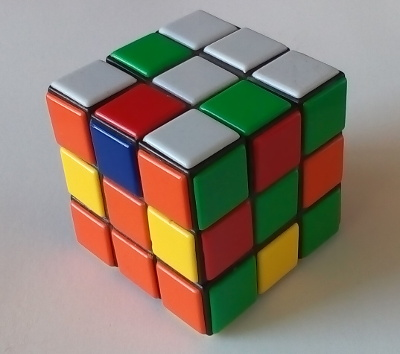
\includegraphics[scale=0.75]{SAT/rubik2/3solved.jpg}
\caption{Rubik's cube as pocket cube}
\end{figure}

\subsubsection{Some discussion}

\url{https://news.ycombinator.com/item?id=15214439},\\
\url{https://www.reddit.com/r/compsci/comments/6zb34i/solving_pocket_rubiks_cube_222_using_z3_and_sat/},\\
\url{https://www.reddit.com/r/Cubers/comments/6ze3ua/theory_dennis_yurichev_solving_pocket_rubiks_cube/}.


\subsection{List of SAT-solvers}

% TODO authors, URLs

\begin{itemize}

\item MiniSat\footnote{http://minisat.se/}, serving as a base for others

\item PicoSat, PrecoSat, Lingeling. Created by Armin Biere. Plingeling supports multithreading.

\item CryptoMiniSat. Created by Mate Soos for cryptographical problems exploration.
Supports XOR clauses, multithreading.
Has Python API.

\end{itemize}



